% This is a template for Ph.D. dissertations in the UCI format.
%
% All fonts, including those for sub- and superscripts, must be 10
% points or larger.  Recommended sizes are 14-point for chapter
% headings, 12-point for the main body of text and figure/table
% titles, and 10-point for footnotes, sub- and super-scripts, and text
% in figures and tables.
%
% Notes: Add short title to figures, sections, via square brackets,
% e.g. \section[short]{long}.
%
\documentclass[12pt,fleqn]{ucithesis}

% A few common packages
\usepackage{amsmath}
\usepackage{amsthm}
\usepackage{array}
\usepackage{graphicx}
\usepackage{natbib}
\usepackage{relsize}

% Some other useful packages
\usepackage{caption}
\usepackage{subcaption}  % \begin{subfigure}...\end{subfigure} within figure
\usepackage{multirow}
\usepackage{tabularx}

% plainpages=false fixes the "duplicate ignored" error with page counters
% Set pdfborder to 0 0 0 to disable colored borders around PDF hyperlinks
\usepackage[plainpages=false,pdfborder={0 0 0}]{hyperref}

% Uncomment the following two lines to use the algorithm package,
% which provides an algorithm environment similar to figure and table
% ("\begin{algorithm}...\end{algorithm}"). A list of algorithms will
% automatically be added in the preliminary pages. Note that you
% probably want a package for the actual code to go with this (e.g.,
% algorithmic).
%\usepackage{algorithm}
%\renewcommand{\listalgorithmname}{\protect\centering\protect\Large LIST OF ALGORITHMS}

% Uncomment the following line to enable Unicode support. This will allow you
% to enter non-ASCII characters (such as accented characters) directly without
% having to use LaTeX's awkward escape syntax (e.g., \'{e})
% NOTE: You may have to install the ucs.sty package for this to work. See:
% http://www.unruh.de/DniQ/latex/unicode/
%\usepackage[utf8x]{inputenc}

% Uncomment the following to avoid "widowing", where page breaks cause
% single lines of paragraphs to float onto the next page (this is not
% a UCI requirement but more of an aesthetic choice).
%\widowpenalty=10000
%\clubpenalty=10000

% Modify or extend these at will.
\newtheorem{theorem}{\textsc{Theorem}}[chapter]
\newtheorem{definition}{\textsc{Definition}}[chapter]
\newtheorem{example}{\textsc{Example}}[chapter]

% Macros for title, author, abstract, etc.
\thesistitle{Efficient Hosted Interpreter for Dynamic Languages}

\degreename{Doctor of Philosophy}

% Use the wording given in the official list of degrees awarded by UCI:
% http://www.rgs.uci.edu/grad/academic/degrees_offered.htm
\degreefield{Computer Engineering}

% Your name as it appears on official UCI records.
\authorname{Wei Zhang}

% Use the full name of each committee member.
\committeechair{Professor Michael Franz}
\othercommitteemembers
{
  Professor Kwei-Jay Lin\\
  Professor Guoqing Xu
}

\degreeyear{2015}

\copyrightdeclaration
{
  Portion of Chapter~\ref{chp:ch3-bytecode} {\copyright} $2013$, $2014$ ACM \\
  Portion of Chapter~\ref{chp:ch4-zippy} {\copyright} $2014$ ACM \\
  Portion of Chapter~\ref{chp:ch5-peeling} {\copyright} $2014$ ACM \\
  All other materials {\copyright} {\Degreeyear} \Authorname
}

% If you have previously published parts of your manuscript, you must list the
% copyright holders; see Section 3.2 of the UCI Thesis and Dissertation Manual.
% Otherwise, this section may be omitted.
% \prepublishedcopyrightdeclaration
% {
% 	Chapter 4 {\copyright} 2003 Springer-Verlag \\
% 	Portion of Chapter 5 {\copyright} 1999 John Wiley \& Sons, Inc. \\
% 	All other materials {\copyright} {\Degreeyear} \Authorname
% }

% The dedication page is optional.
\dedications
{

  To my supporting parents and lovely wife.
}

\acknowledgments
{
  First and foremost, I would like to thank my advisor Professor Michael Franz for his mentorship and support during my years in graduate school.
  I am deeply grateful that he admitted me to his fantastic research group and brought me into the world of programming languages.
  Working under his supervision has been one of my most fulfilling period of my life.

  I would also like to thank Professor Kwei-Jay Lin and Professor Guoqing Xu for accepting to serve on my committee.

  I am deeply grateful for Dr. Stefan Brunthaler and Dr. Per Larsen for closely working with me on this research.
  Their continuous guidance, motivation and insightful comments greatly improve me as a graduate student researcher.
  This thesis would not be possible without their help.

  I would also like to thank Dr. Christian Wimmer for his valuable feedback to my work and mentorship during my internships at Oracle Labs.
  I am also grateful to Chris Seaton, Andreas Woess and other people I have worked with at Oracle Labs.
  Their mastery on software design deeply inspired me.

  Lastly, I would like to thank my amazing colleagues.
  I have been fortunate to be a part of this great research group.
  My thanks go to: Mason Chang, Todd Jackson, Michael Bebenita, Christoph Kerschbaumer, Gregor Wagner, Eric Hennigan, 
  Andrei Homescu, G{\"u}lfem Savrun-Yeniçeri, Stephen Crane, Mark Murphy, Codru\c{t} Stancu, Mohaned Qunaibit, Brian Belleville and Julian Lettner.
}


% Some custom commands for your list of publications and software.
\newcommand{\mypubentry}[3]{
  \begin{tabular*}{1\textwidth}{@{\extracolsep{\fill}}p{4.5in}r}
    \textbf{#1} & \textbf{#2} \\
    \multicolumn{2}{@{\extracolsep{\fill}}p{.95\textwidth}}{#3}\vspace{6pt} \\
  \end{tabular*}
}
\newcommand{\mysoftentry}[3]{
  \begin{tabular*}{1\textwidth}{@{\extracolsep{\fill}}lr}
    \textbf{#1} & \url{#2} \\
    \multicolumn{2}{@{\extracolsep{\fill}}p{.95\textwidth}}
    {\emph{#3}}\vspace{-6pt} \\
  \end{tabular*}
}

% Include, at minimum, a listing of your degrees and educational
% achievements with dates and the school where the degrees were
% earned. This should include the degree currently being
% attained. Other than that it's mostly up to you what to include here
% and how to format it, below is just an example.
\curriculumvitae
{

\textbf{EDUCATION}

  \begin{tabular*}{1\textwidth}{@{\extracolsep{\fill}}lr}
    \textbf{Doctor of Philosophy in Computer Engineering} & \textbf{2015} \\
    \vspace{6pt}
    University of California, Irvine & \emph{Irvine, California} \\

    \textbf{Master of Science in Computer Engineering} & \textbf{2010} \\
    \vspace{6pt}
    Chalmers University of Technology & \emph{Gothenburg, Sweden} \\

    \textbf{Bachelor of Science in Mechanical Engineering} & \textbf{2004} \\
    \vspace{6pt}
    University of Science and Technology Beijing & \emph{Beijing, China} \\
  \end{tabular*}

\vspace{12pt}
\textbf{RESEARCH EXPERIENCE}

  \begin{tabular*}{1\textwidth}{@{\extracolsep{\fill}}lr}
    \textbf{Graduate Student Researcher} & \textbf{2010--2015} \\
    \vspace{6pt}
    University of California, Irvine & \emph{Irvine, California} \\

    \textbf{Master Student Researcher} & \textbf{2010} \\
    \vspace{6pt}
    Chalmers University of Technology & \emph{Gothenburg, Sweden} \\
  \end{tabular*}

\vspace{12pt}
\textbf{PROFESSIONAL EXPERIENCE}

  \begin{tabular*}{1\textwidth}{@{\extracolsep{\fill}}lr}
    \textbf{Software Development Intern} & \textbf{Summer 2014} \\
    \vspace{6pt}
    Oracle Labs & \emph{Belmont, CA} \\

    \textbf{Software Development Intern} & \textbf{Summer 2013} \\
    \vspace{6pt}
    Oracle Labs & \emph{Belmont, CA} \\

    \textbf{Customer Service Engineer} & \textbf{2007--2008} \\
    \vspace{6pt}
    ASML & \emph{Shanghai, China} \\

    \textbf{Production Engineer} & \textbf{2005--2007} \\
    \vspace{6pt}
    AT\&S & \emph{Shanghai, China} \\

    \textbf{Mechanical Design Engineer} & \textbf{2004--2005} \\
    \vspace{6pt}
    BMEI & \emph{Beijing, China} \\
  \end{tabular*}

\pagebreak

\textbf{PUBLICATIONS}

  % \mypubentry{Awesome paper}{Jun 2011}{Conference name}
  % \mypubentry{Another awesome paper}{Aug 2012}{Conference name}

Wei Zhang, Per Larsen, Stefan Brunthaler, Michael Franz.
\textbf{Accelerating Iterators in Optimizing AST Interpreters}.
\textit{In Proceedings of the 29th ACM SIGPLAN Conference on Object Oriented Programming:
Systems, Languages, and Applications, Portland, OR, USA, October 20-24, 2014 (OOPSLA '14)}, 2014.

G{\"u}lfem Savrun-Yeniçeri, Wei Zhang, Huahan Zhang, Eric Seckler, Chen Li, Stefan Brunthaler,
Per Larsen, Michael Franz.
\textbf{Efficient Hosted Interpreters on the JVM}.
\textit{In ACM Transactions on Architecture and Code Optimization, volume 11(1) pages 9:1–9:24}, 2014.

G{\"u}lfem Savrun-Yeniçeri, Wei Zhang, Huahan Zhang, Chen Li, Stefan Brunthaler, Per Larsen, Michael Franz.
\textbf{Efficient Interpreter Optimizations for the JVM}.
\textit{In Proceedings of the 10th International Conference on Principles and Practice of Programming in Java,
Stuttgart, Germany, September 11-13, 2013 (PPPJ '13)}, 2013.

\vspace{12pt}
\textbf{SOFTWARE}

\mysoftentry{ZipPy}{http://bitbucket.org/ssllab/zippy/}
{A fast and lightweight Python 3 implementation built using the Truffle framework.
It leverages the underlying Java JIT compiler and compiles Python programs to highly optimized machine code at runtime.}

\mysoftentry{ModularVM}{https://bitbucket.org/thezhangwei/modularvm/}
{An extension to the Maxine VM (Java Virtual Machine) that enables deeper integrations with JVM languages
like Jython (Python), Rhino (JavaScript) or JRuby (Ruby). It automatically accelerates guest language interpreters written in Java.}

}

% The abstract should not be over 350 words, although that's
% supposedly somewhat of a soft constraint.
\thesisabstract
{

Motivated by high development costs, production compilers and virtual machines, often support more than one language.
This strategy is most effective when the language family is homogeneous.
Many languages are very amenable to static program analysis, however, dynamic languages are not.
Consequently, a single VM cannot deliver peak performance for both types of languages without adapting its optimization strategy accordingly.

Informally, we host a ``highly dynamic'' language (Python) on the Java Virtual Machine, a VM for ``moderately dynamic'' languages.
While we are not the first to do so, our approach diverges from current practice by representing Python programs as abstract syntax trees, ASTs, rather than bytecode.
Not only are ASTs the simplest and most natural programming language implementation,
they also lend themselves well to optimizations those are particularly beneficial to highly dynamic languages.
Compared to Jython, which compiles Python programs to Java bytecode, our Python prototype is faster and requires less implementation effort.

}


%%% Local Variables: ***
%%% mode: latex ***
%%% TeX-master: "thesis.tex" ***
%%% End: ***


% Add PDF document info fields
\hypersetup{
	pdftitle={\Thesistitle},
	pdfauthor={\Authorname},
	pdfsubject={\Degreefield},
}

% Uncomment the following to have numbered subsubsections (by default
% numbering goes only to subsections).
%\setcounter{secnumdepth}{4}


% Set this to only select a subset of the includes directives below.
% Very handy to speed up compilation if you're working on a certain
% part of your thesis. It conserves page numbers, references, etc.
% even for non-included files.
%\includeonly{chapter1}

\begin{document}

% Preliminary pages are always loaded (TOC, CV, etc.)
\preliminarypages

% Include the different components of your thesis, in separate files.
% Using \include allows you to set \includeonly above.
\chapter{Introduction}

This is an example using the \LaTeX{} template for UCI theses and
dissertation documents \cite{uci-thesis-latex}. Figure
\ref{fig:sourcecode} is just for illustration purposes, as is Table
\ref{tab:coordinates}.

\begin{figure}
\begin{verbatim}
#include <iostream>
int main(int argc, char** argv) {
  std::cout << "Hello World." << std::endl;
  return 0;
}
\end{verbatim}
  \caption{Example source code.}
  \label{fig:sourcecode}
\end{figure}

\section{Background}

Lorem ipsum dolor sit amet, consectetur adipisicing elit, sed do
eiusmod tempor incididunt ut labore et dolore magna aliqua. Ut enim ad
minim veniam, quis nostrud exercitation ullamco laboris nisi ut
aliquip ex ea commodo consequat. Duis aute irure dolor in
reprehenderit in voluptate velit esse cillum dolore eu fugiat nulla
pariatur. Excepteur sint occaecat cupidatat non proident, sunt in
culpa qui officia deserunt mollit anim id est laborum.

\begin{table}
  \centering
  \begin{tabular}{|rr|r|}
    \hline
    $x$ & $y$ & $z$ \\
    \hline
    14 & 12 & -2 \\
    0 & 33 & -25 \\
    -3 & 11 & 22 \\
    4 & 4 & 6 \\
    \hline
  \end{tabular}
  \caption{Example coordinates.}
  \label{tab:coordinates}
\end{table}

Lorem ipsum dolor sit amet, consectetur adipisicing elit, sed do
eiusmod tempor incididunt ut labore et dolore magna aliqua. Ut enim ad
minim veniam, quis nostrud exercitation ullamco laboris nisi ut
aliquip ex ea commodo consequat. Duis aute irure dolor in
reprehenderit in voluptate velit esse cillum dolore eu fugiat nulla
pariatur. Excepteur sint occaecat cupidatat non proident, sunt in
culpa qui officia deserunt mollit anim id est laborum.


%%% Local Variables: ***
%%% mode: latex ***
%%% TeX-master: "thesis.tex" ***
%%% End: ***

\chapter{Hosted Bytecode Interpreter}

A programming language interpreter executes programs in two steps.
First it parses the human readable source code, verifies its correctness and translates the code into a more efficient intermediate representation (IR) format.
The interpreter then picks up the translated program and executes it piece by piece.

Bytecode interpreters parse source program into bytecode, a highly compressed representation of the program.
The format of the bytecode is a form of virtual instruction set designed for this particular interpreter.
In the second step bytecode interpreters execute the bytecode as a sequence of virtual instruction one instruction at a time before finishing the last one.
Interpreters are also regard as virtual machines, since they emulate ``machines'' with their own virtual instruction sets.

In this Chapter, we go over performance overheads of bytecode interpreters and the classic techniques used to minimize these overheads.
Lastly, we introduce ModularVM~\cite{savrun2013, savrun2014}, a research JVM that automatically optimize the performance of hosted bytecode interpreters.

\section{Performance Anatomy of Bytecode Interpreters}

Bytecode interpreters execute bytecode one instruction at a time.
For each instruction, the interpretation consists of three steps~\cite{davis2003case}:
\begin{itemize}
  \item Instruction dispatch
  \item Operand access
  \item Performing the function of the instruction
\end{itemize}
Instruction dispatch includes fetching the next instruction, decoding the instruction and transferring program execution to the actual implementation of the instruction.
Operand access involves fetching operands required to perform the instruction from either a temporal operand stack or a virtual register file depending on the design of the virtual instruction set.
It also includes storing the computed result back to where temporal operands should be stored.
Subsequently in the last step the interpreter performs the actual computation.
For instance, if the instruction is addition of two numbers, the actually addition is performed in this step.

\begin{figure}[th]
\centering
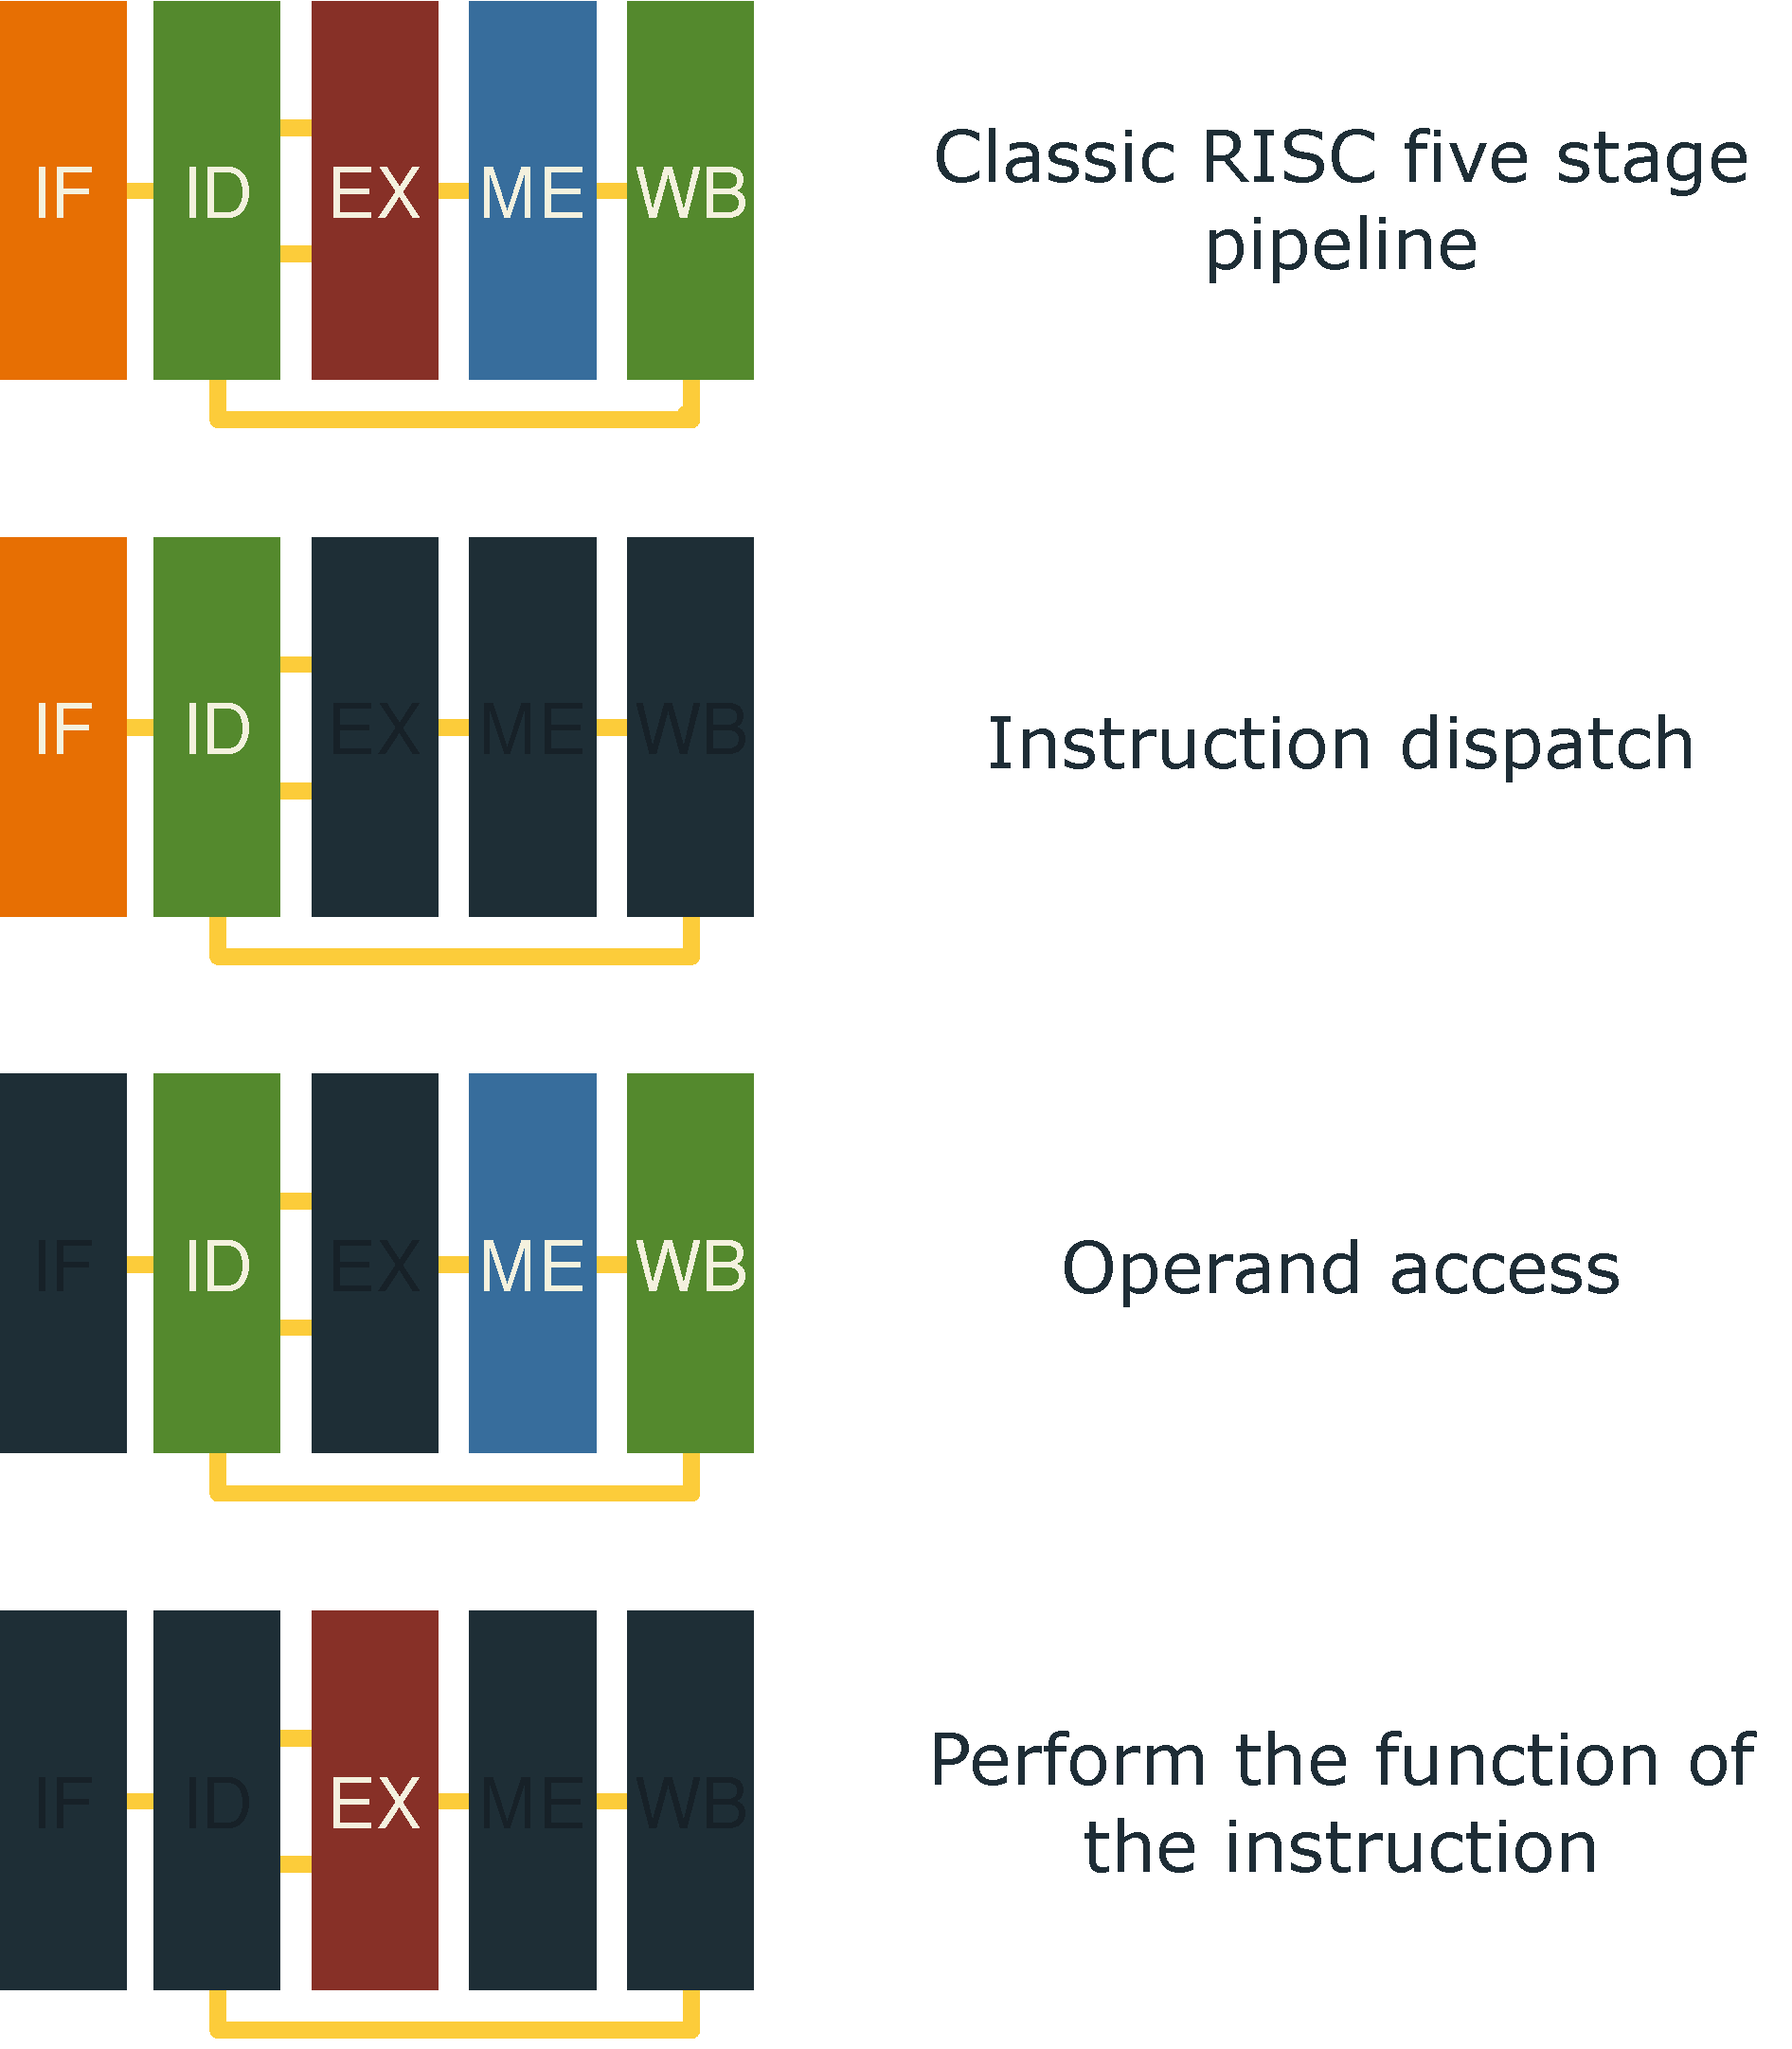
\includegraphics[scale=.25]{figures/ch2-risc-pipeline.pdf}
\caption{Interpretation costs of bytecode interpreters}
\label{fig:interpretation-cost}
\end{figure}

An interesting way to further illustrate the purpose of each interpretation step
from the angle of a virtual machine is to correlate them with the stages in a classic reduced instruction set computer (RISC) pipeline.
Figure~\ref{fig:interpretation-cost} illustrates the five stages in a classic RISC pipeline:
instruction fetch (IF), instruction decode (ID), execute (EX), memory access (ME) and write back (WB).
The instruction dispatch step in bytecode interpreters is similar to instruction fetch and decode stages in RISC.
We can correlate the late stage of instruction decode, memory access and write back in RISC to operand access in an interpreter.
Since these are the stages that prepare the operands for the computing unit and stores the end result back to either a register or memory address.
The interpreter step that performs the function of the instruction works exactly as the execute stage in RISC, which performs the actual computation.

The cost of running a hosted program on an interpreter consists of the costs of performing each of the three steps we described above.
Among those steps, instruction dispatch and operand access does not directly contribute to the actual work of the hosted program.
The less time the interpreter spend in these two steps, the more time the interpreter spend in doing the actual work.
Therefore, an efficient bytecode interpreter must encompass techniques that optimize instruction dispatch and operand access.

\subsection{Switch-based Dispatch}

\begin{figure}[th]
\centering
\subfigure[dispatch loop] {
  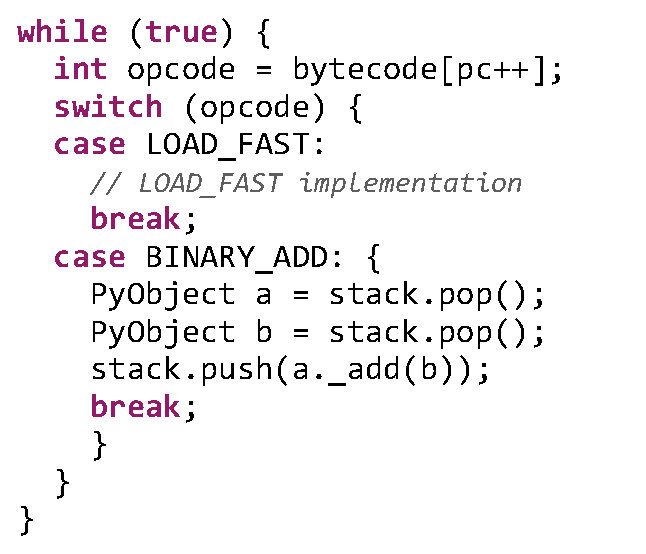
\includegraphics[scale=.70]{figures/ch2-switch-based-dispatch-code.pdf}
  \label{fig:switch-based-dispatch-code}
}
\subfigure[branches in switch-based dispatch] {
  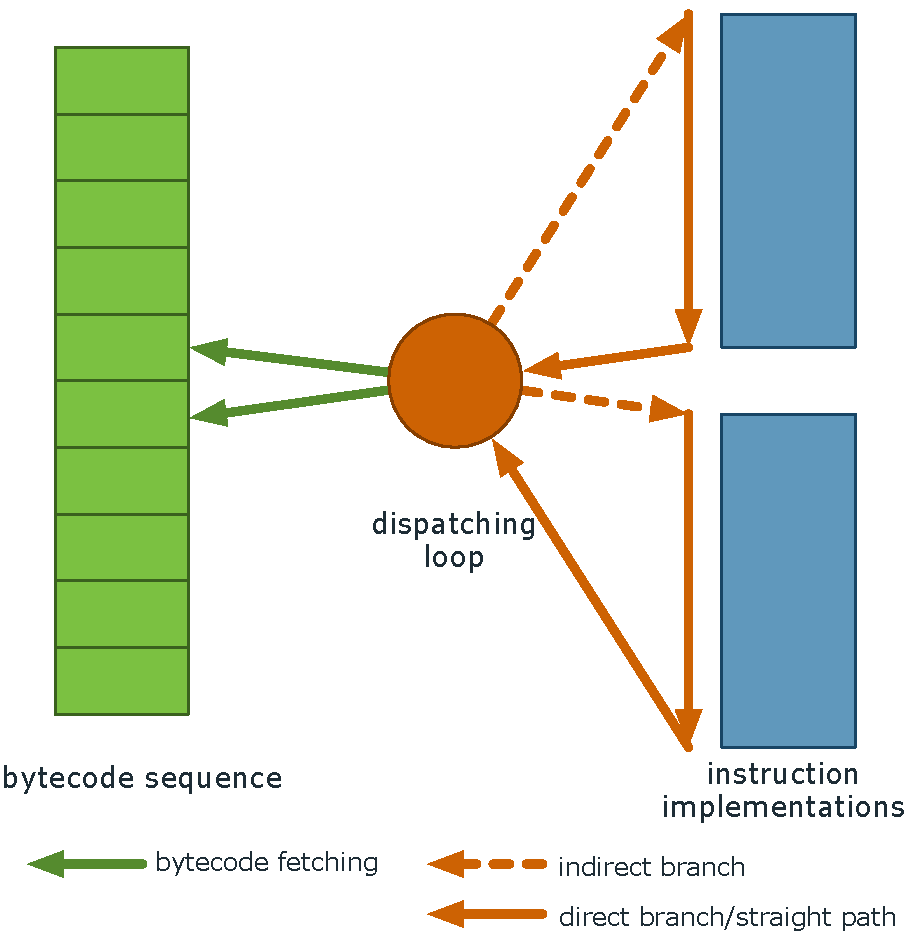
\includegraphics[scale=.47]{figures/ch2-switch-based-dispatch-branch.pdf}
  \label{fig:switch-based-dispatch-branch}
}
\caption{switch-based dispatch}
\label{fig:switch-based-dispatch}
\end{figure}

The simplest way to construct a bytecode interpreter is to use an interpreter loop and a switch statement in the loop to dispatch each bytecode instruction.
Figure~\ref{fig:switch-based-dispatch-code} illustrates a switch-based bytecode interpreter loop written in Java.
In each iteration of the loop, the interpreter fetches the next instruction and use the switch statement to redirect execution to the case block that implements the instruction.
Figure~\ref{fig:switch-based-dispatch-branch} shows the branches involved in a switch-based dispatch.
Note that each iteration of the dispatch loop shares the same indirect branch.
Since the bytecode sequence is input dependent and unlikely to form a predictable pattern,
branch prediction mechanisms in modern hardware tend to mis-predict the shared indirect branch.
This mis-prediction results in a significant performance penalty for switch-based bytecode interpreters.

\section{Efficient Instruction Dispatch Techniques}
\label{sec:efficient-instruction-dispatch-techniques}

\subsection{Direct Threading Dispatch}
\label{sec:direct-threading-dispatch}

\begin{figure}[th]
\centering
\subfigure[direct threading interpreter] {
  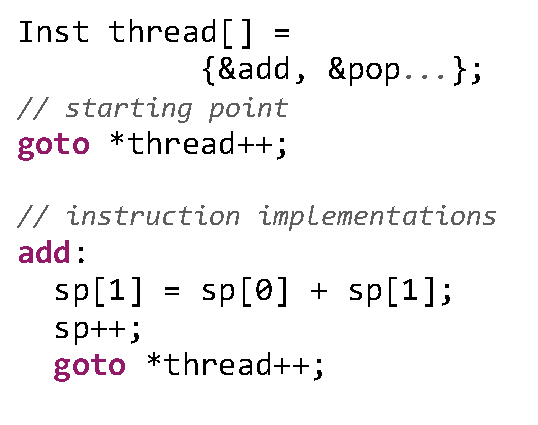
\includegraphics[scale=.85]{figures/ch2-direct-threading-dispatch-code.pdf}
  \label{fig:direct-threading-dispatch-code}
}
\subfigure[branches in direct threading dispatch] {
  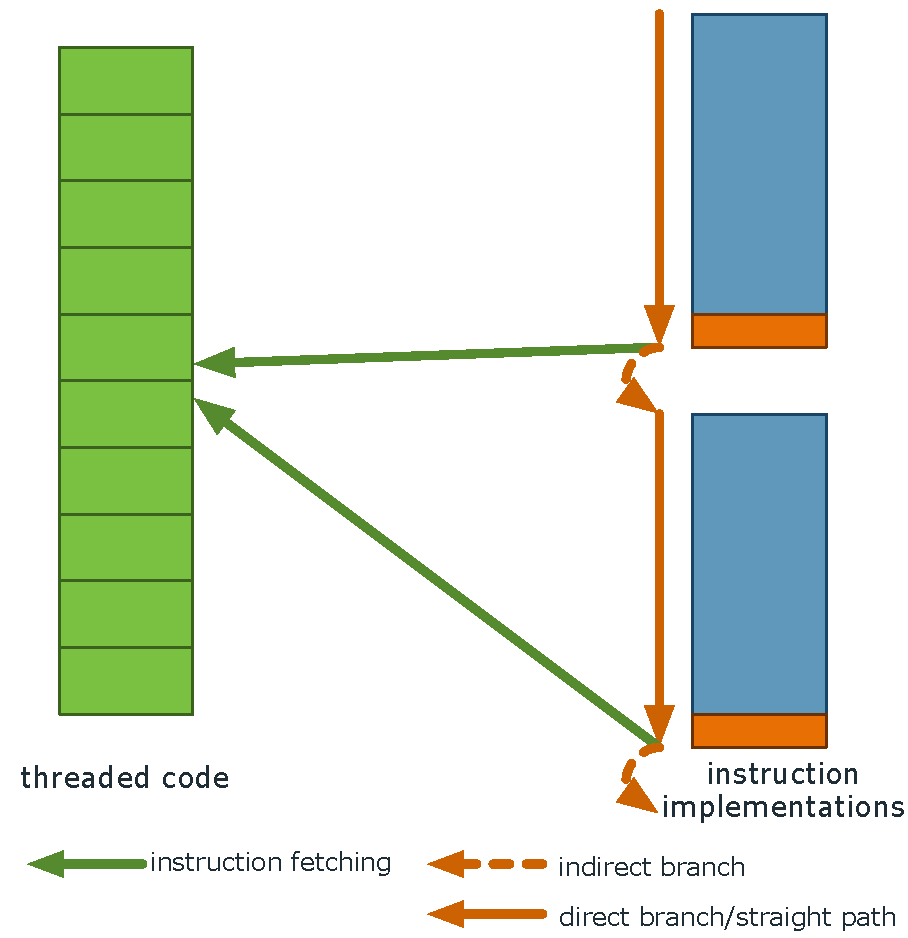
\includegraphics[scale=.47]{figures/ch2-direct-threading-dispatch-branch.pdf}
  \label{fig:direct-threading-dispatch-branch}
}
\caption{direct threading dispatch}
\label{fig:direct-threading-dispatch}
\end{figure}

Instead of letting each instruction dispatch share the same branch, direct threading duplicates instruction dispatch at the end of each instruction implementation~\cite{bell73}.
Figure~\ref{fig:direct-threading-dispatch-code} illustrates this technique written in C.
Direct threading requires an additional translation phase that translates the bytecode sequence into a sequence of pointers or the threaded code.
Each pointer in the threaded code points to the instruction implementation that corresponds to the bytecode instruction in the original bytecode input.
The interpreter starts interpretation by jumping to the address pointed by the first pointer in the threaded code as shown in Figure~\ref{fig:direct-threading-dispatch-code}.
Similarly each instruction implementation repeat the same dispatch routine at the end of it to forward execution to the next instruction implementation.
The duplicated dispatch branches reduce indirect branch mis-predictions.
Therefore, direct threading alleviates the performance loss we have seen in switch-based dispatch.

\subsection{Subroutine Threading Dispatch}

\begin{figure}[th]
\centering
\subfigure[subroutine threaded code] {
  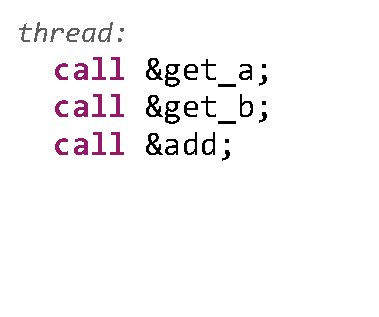
\includegraphics[scale=.85]{figures/ch2-subroutine-threading-dispatch-code.pdf}
  \label{fig:subroutine-threading-dispatch-code}
}
\subfigure[branches in subroutine threading dispatch] {
  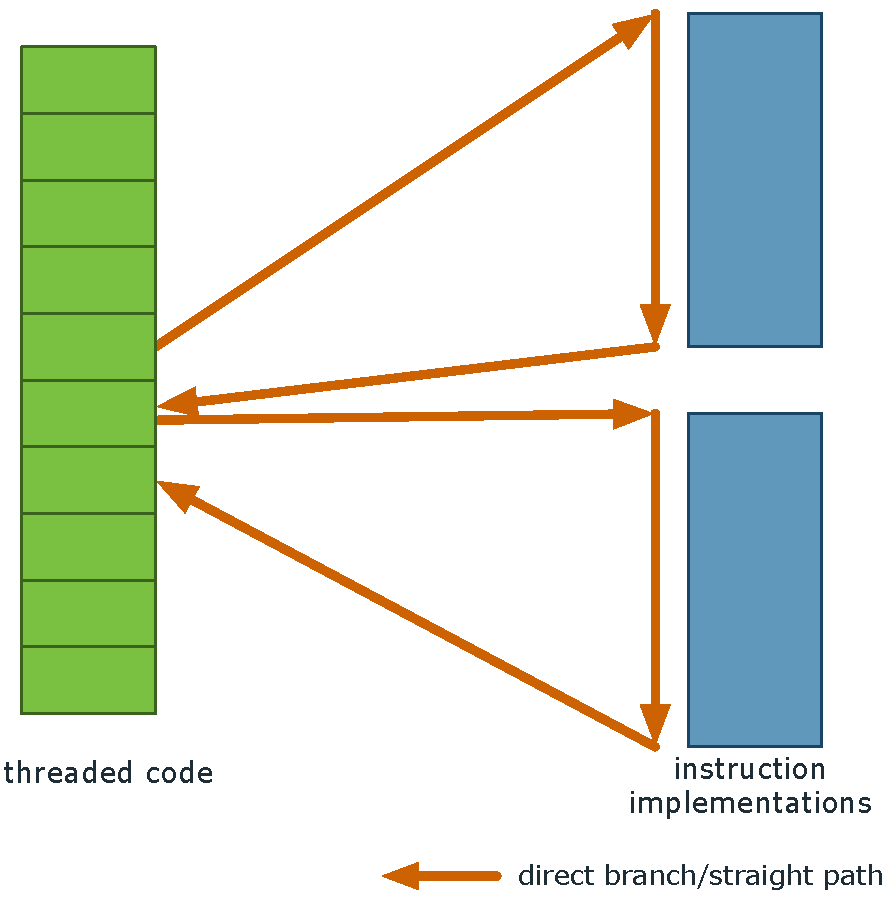
\includegraphics[scale=.47]{figures/ch2-subroutine-threading-dispatch-branch.pdf}
  \label{fig:subroutine-threading-dispatch-branch}
}
\caption{subroutine threading dispatch}
\label{fig:subroutine-threading-dispatch}
\end{figure}

Subroutine threading takes one step further by translating the input bytecode sequence directly to executable machine code.
The translated machine code or the subroutine threaded code is a sequence of machine level calls.
Each call is a direct branch jumping to an instruction implementation as a subroutine.
The subroutine threaded code translation phase translates each input bytecode to a subroutine call to the corresponding instruction implementation.
Each instruction implementation ends with a return instruction that transfer execution back to the threaded code.
Note that the call instruction in subroutine threading is a direct branch.
Although the return instruction is an indirect branch, modern hardware can accurately predict call/return repairs which results in a performance increase.

\section{Efficient Instruction Dispatch for Hosted Bytecode Interpreters}

Instruction dispatch greatly affects the overall performance of a bytecode interpreter.
The implementation of an efficient instruction dispatch technique like the ones explained in Chapter~\ref{sec:efficient-instruction-dispatch-techniques}
relies on the use of computed goto's.
Due to the restricted use of pointers, a hosted bytecode interpreter written in Java can not make use of those techniques.
To address this issue, we extend the JVM by adding the functionality of threaded code generation to enable efficient instruction dispatch for hosted interpreters.
Our research prototype takes an existing switch-based bytecode interpreter written in Java, and converts it into a direct threading interpreter in a semi-automatic fashion.

\subsection{System Overview}

\begin{figure}[th]
\centering
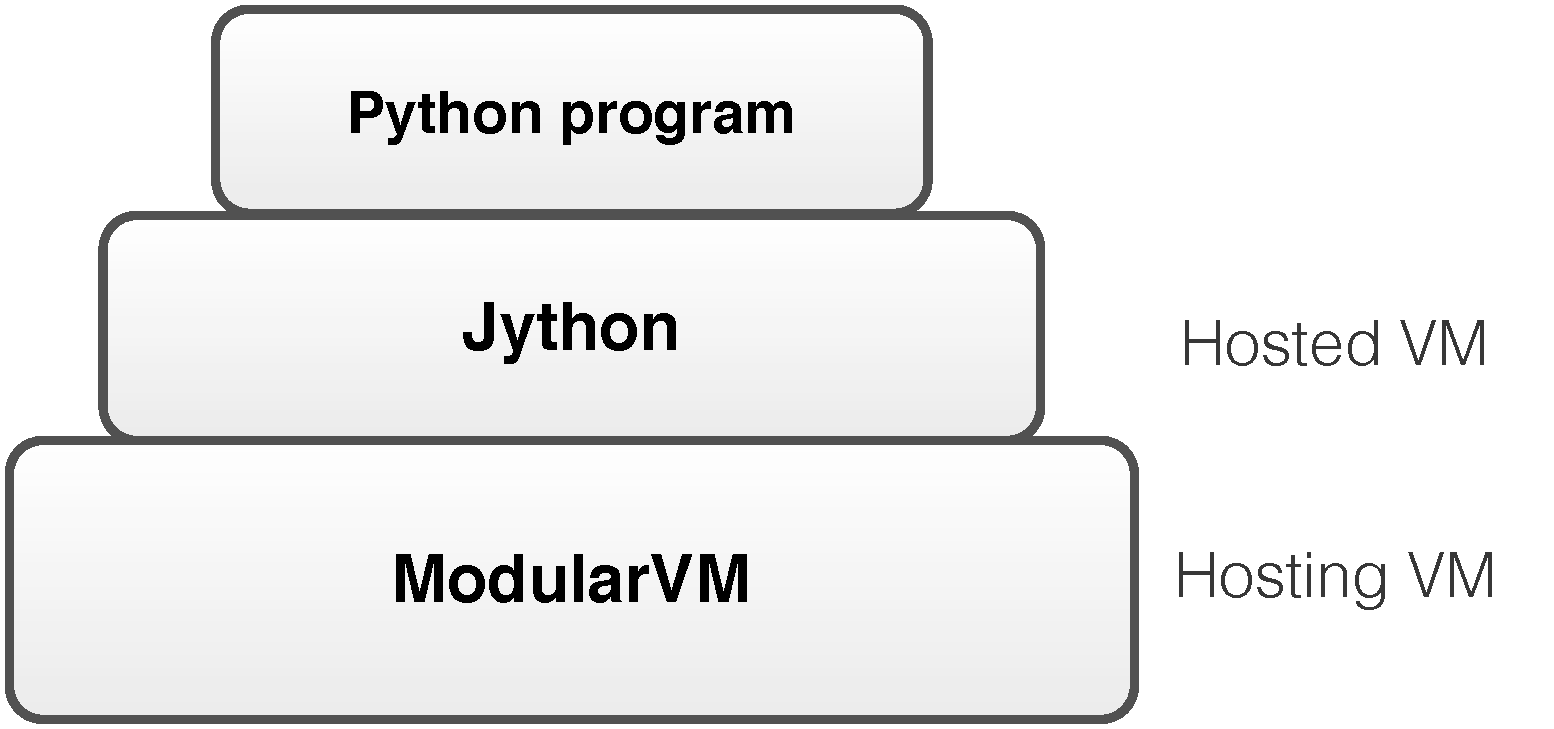
\includegraphics[scale=.3]{figures/ch2-jython-on-modularvm.pdf}
\caption{Jython on ModularVM}
\label{fig:jython-on-modularvm}
\end{figure}

Our system, Modular VM, is an extension to Maxine VM~\cite{Wimmer2013}, a research JVM developed at Oracle Labs.
We build Modular VM with the ability to recognize hosted interpreters running on top of it and automatically optimizes them.
We host Jython, a Python VM written in Java, on Modular VM in our experiment to show case our optimization.
Figure~\ref{fig:jython-on-modularvm} illustrates the overall system setup.
Modular VM hosts Jython like other regular JVMs.
Jython executes Python program in two fashions: using the baseline bytecode interpreter or
compiling Python code to Java bytecode and let the JVM compiler further compile it down to machine code.
Our optimization focuses on the bytecode interpreter.
It shows that by incorporating efficient interpreter optimizations, bytecode interpreter can deliver comparable performance to a basic compiler.

\subsection{Threaded Code Generation}

\begin{figure}[!h]
\centering
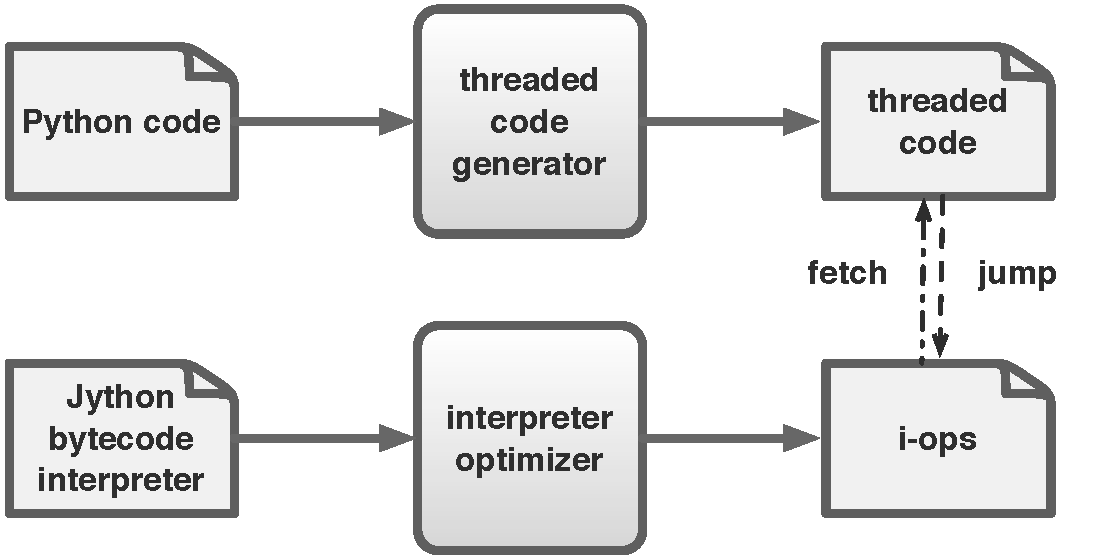
\includegraphics[scale=.5]{figures/ch2-direct-threading-on-modularvm.pdf}
\caption{Threaded code generation}
\label{fig:direct-threading-on-modularvm}
\end{figure}

Modular VM performs threaded code generation in two steps.
First, it recognizes the hosted interpreter running on top of it and transforms it into an optimized one.
To be more specific, Modular VM extracts all the bytecode instruction implementations or i-ops for short from the interpreter and
compiles them into machine code using the existing Java compiler.
Modular VM then initializes an i-op code table that contains the address of all the compiled i-ops.
After this transformation, the interpreter is ready to execute Python programs.
It first translates Python source code to Python bytecode and then further translates bytecode to direct threaded code using the i-op code table.
The generated threaded code is a sequence of code pointers copied from the i-op code table.

Figure~\ref{fig:direct-threading-on-modularvm} illustrates this work flow.
The interpreter optimizer in the Figure applies the transformation to Jython's bytecode interpreter.
Subsequently, the thread code generator produces threaded code and executes it.
Both interpreter optimizer and threaded code generator are part of Modular VM.
Our system encapsulates the details of i-ops compilation and threaded code generation from the hosted VM.

\subsubsection{Interpreter Annotation}

\begin{figure}[ht]
\centering
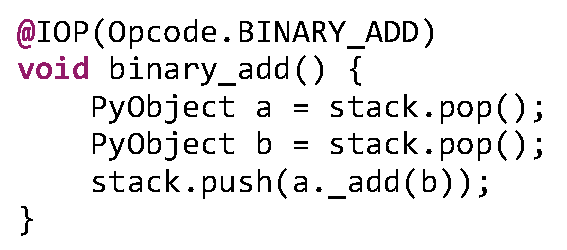
\includegraphics[scale=.65]{figures/ch2-annotated-iop-code.pdf}
\caption{Annotated i-op}
\label{fig:annotated-iop}
\end{figure}

Modular VM uses a Java annotation based domain specific language to integrate with the hosted interpreter.
Our programmable interface provides a set of annotations for hosted VM implementers to annotate different components of their interpreter.
We expect hosted VM implementers to properly annotate the interpreter class, the bytecode class and all the i-op methods for our system to identify the structure of the interpreter.
Figure~\ref{fig:annotated-iop} shows an annotated i-op in Jython's bytecode interpreter refactored to its own separate method.
Modular VM automatically picks up Java methods annotated as i-ops, optimizes them and put them into the i-op code table.

\subsubsection{Next Dispatch}

\begin{figure}[ht]
\centering
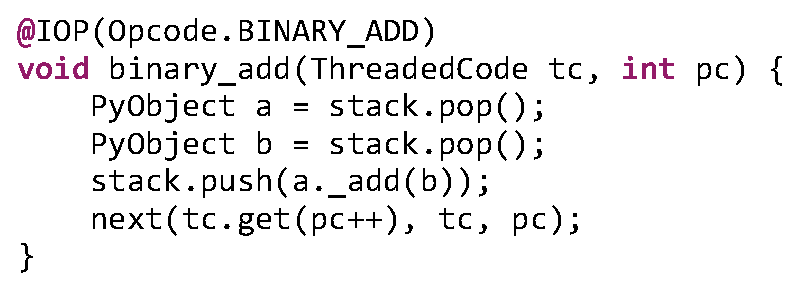
\includegraphics[scale=.65]{figures/ch2-iop-with-next-code.pdf}
\caption{I-op with next dispatch}
\label{fig:iop-with-next}
\end{figure}

Direct threading, as explained in Chapter~\ref{sec:direct-threading-dispatch}, duplicates instruction dispatch at the end of each instruction implementation or i-op.
When the interpreter optimizer compiles an i-op, it also insert a synthesized \emph{next} routine at the end of the i-op.
The \emph{next} routine performs the actual instruction dispatch.
Figure~\ref{fig:iop-with-next} illustrates the i-op of \texttt{BINARY\_ADD} in Jython with the \emph{next} routine.
Note that the figure shows what the program looks like with the added instruction dispatch.
Hosted VM implementers are not required to write the additional code.
As shown in Figure~\ref{fig:iop-with-next}, the intrinsic function \texttt{next} performs an indirect jump to the next i-op in the threaded code.
The \emph{next} routine also passes the reference to the threaded code and virtual program pointer to the next instruction to continue the execution of the program.

\subsubsection{Stack Frame Reusing}

As described above, the \texttt{next} instruction dispatch performs a native indirect branch instead of a call.
Therefore, i-ops need to reuse the same stack frame allocated for each Python function invocation.
We implement this using two special i-ops, \texttt{PROLOGUE} and \texttt{EPILOGUE}.
Both of them are manually assembled instead of compiled from Java source code.
\texttt{PROLOGUE}, used at the beginning of a function, allocates a stack frame that is big enough to accommodate all i-ops.
\texttt{EPILOGUE}, used to model \texttt{RETURN}, deallocates the stack frame and returns.
The interpretation of a Python method always start with a \texttt{PROLOGUE} and end with an \texttt{EPILOGUE}.
Stack frame reusing reduces the number of native machine instructions executed for each hosted virtual machine instruction dispatch.

\subsubsection{Efficient Array Stores}
\label{sec:efficient-array-stores}

Another problem affecting hosted interpreter performance on the JVM is the performance of array stores.
Java being a safe language performs type check such as \texttt{ArrayStoreException} checks on array stores.
Hosted language interpreters like the one in Jython uses an operand stack to manage temporal operands.
Internally, the operand stack is implemented as an Java object array.
During interpretation, every i-op that produces a value performs an array store onto the operand stack.
As a result, the interpreter repeatedly performs the same the type check, even though every i-op is guaranteed to produce an value that is safe to be stored on the operand stack.

We identified the detrimental effect of preserving array type-safety for hosted interpreters.
Our interpreter optimizer omits the \texttt{ArrayStoreException} checks when compiling the i-ops of hosted interpreters.

\subsubsection{An Example}

\begin{figure}[th]
\centering
\subfigure[Python source code] {
  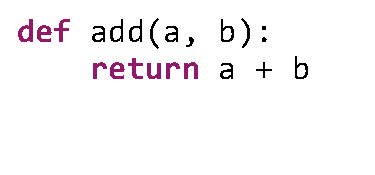
\includegraphics[scale=.85]{figures/ch2-threaded-code-example-python.pdf}
  \label{fig:threaded-code-example-python}
}
\subfigure[Python bytecode] {
  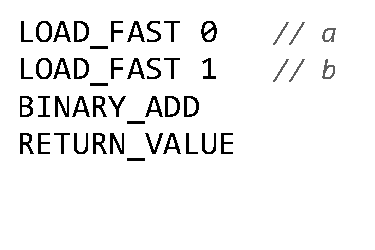
\includegraphics[scale=.75]{figures/ch2-threaded-code-example-bytecode.pdf}
  \label{fig:threaded-code-example-bytecode}
}
\subfigure[Threaded code] {
  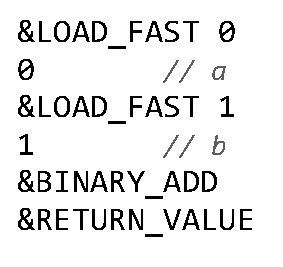
\includegraphics[scale=.7]{figures/ch2-threaded-code-example-threaded-code.pdf}
  \label{fig:threaded-code-example-threaded-code}
}
\caption{Direct threading example}
\label{fig:threaded-code-example}
\end{figure}

Figure~\ref{fig:threaded-code-example} illustrates the Python program translation in Jython hosted on Modular VM.
The input program, as shown in Figure~\ref{fig:threaded-code-example-python}, is a simple Python method that adds two parameters.
Jython first converts the program to the bytecode sequence show in Figure~\ref{fig:threaded-code-example-bytecode}.
Note that the bytecode instruction \texttt{LOAD\_FAST} consists of not only the \texttt{LOAD\_FAST} opcode itself but also an opcode argument ($0$ or $1$) in the bytecode sequence.
Figure~\ref{fig:threaded-code-example-threaded-code} shows the direct threading code produced by the threaded code generator.
Aside from the translated i-op addresses, the threaded code generator also copies opcode arguments, like the one in \texttt{LOAD\_FAST}, into the threaded code.

\section{Evaluation}

% ... and so on

% These commands fix an odd problem in which the bibliography line
% of the Table of Contents shows the wrong page number.
\clearpage
\phantomsection

% "References should be formatted in style most common in discipline",
% abbrv is only a suggestion.
\bibliographystyle{abbrv}
\bibliography{thesis}

% The Thesis Manual says not to include appendix figures and tables in
% the List of Figures and Tables, respectively, so these commands from
% the caption package turn it off from this point onwards. If needed,
% it can be re-enabled later (using list=yes argument).
\captionsetup[figure]{list=no}
\captionsetup[table]{list=no}

% If you have an appendix, it should come after the references.
\include{appendix}

\end{document}
